\documentclass{beamer}

%style
\mode<presentation>
\usetheme{Boadilla}

%Packages
\usepackage[utf8]{inputenc}
\usepackage[ngerman]{babel}
\usepackage{graphicx}
\usepackage{booktabs}
\usepackage{mathtools}
\usepackage{amsmath}
\usepackage{listings}
\usepackage[utf8]{inputenc}
\usepackage[ngerman]{babel}
\usepackage[T1]{fontenc}
\usepackage{lmodern}
\usepackage{tabto}
\usepackage{listings}
\usepackage{framed} 
\usepackage{xcolor} 
\colorlet{shadecolor}{gray!25}
%bibtex
\usepackage[backend=biber, style=authoryear]{biblatex}
\addbibresource{referenzen.bib}

%Einstellungen der Präsentation
\title[Cybersecurity]{Flubot:\\ Android-Malware verbreitet sich über Fake-Patches\\}
\author{Moritz Rupp}
\institute[MR]{Hochschule Albstadt-Sigmaringen}
\setbeamertemplate{navigation symbols}{}%remove navigation symbols
\date{WS 21/22}

%Beginn der Präsentation
\begin{document}

%Titelseite
\begin{frame}
\titlepage
\end{frame}

\begin{frame}{Leitartikel}
\begin{center}
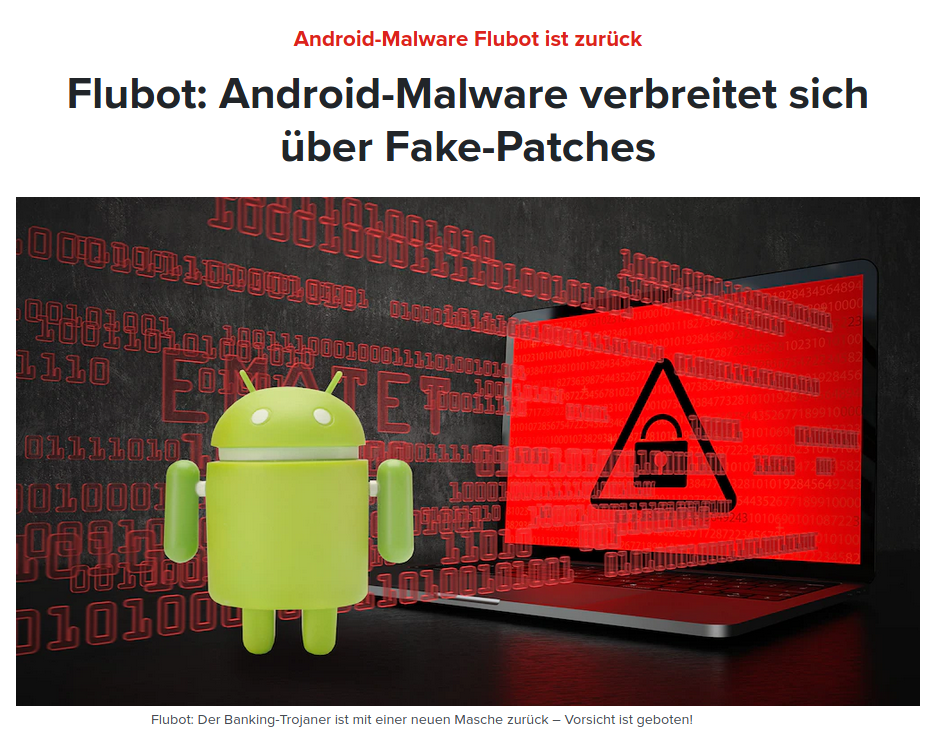
\includegraphics[scale=0.25]{bild.png} \footnote{computerbild.de}

\end{center}

\end{frame}
%Inhaltsverzeichnis
\begin{frame}
\frametitle{Inhalt}
\tableofcontents    
\end{frame}
\section{Terminologie}
\begin{frame}{Terminologie}
\begin{block}{Malware}
Software zu ausführung unerwünschter bzw. schädlicher Funktionen.
\end{block}
\begin{block}{Banking Trojaner}
 Vermeintlich harmlose Anwendung dringt in System ein und greift Daten ab. $\Rightarrow$ Banking Login Daten.
\end{block}
\begin{block}{Phishing}
Vortäuschung von Diensten zu erlangung von Login Informationen.
\end{block}

\begin{block}{Botnetze}
 Große Anzahl an Geräten(Bots) die über Netzwerke automatisiert Malware betreiben.
\end{block}

\end{frame}
\section{Was ist Flubot?}
\begin{frame}{Was ist Flubot?}
\begin{itemize}
 \item Android Malware
 \item Banking Trojaner
 \item Verbreitung über SMS Nachrichten
 \item Nutzung von Botnetzten und Phishing Methoden
 \item Nach wie vor im Umlauf
\end{itemize}

\end{frame}
\begin{frame}{Trivia}
 \section{Trivia}
 \begin{itemize}
 
  \item Erstes Auftreten Ende 2020 in Spanien\\
  	- Frühjar 2021 in Deutschland
  \item Weltweite Verbreitung im laufe des Jahres 2021
  \item \raisebox{-0.9ex}{\~{}}13 Millionen Infizierte Geräte
  \item Finanzieller Schaden schwer festellbar \raisebox{-0.9ex}{\~{}} 8 stelligem Bereich!
 \end{itemize}
\end{frame}

\section{Funktionsweiße}
\begin{frame}{Funktionsweiße}
\begin{itemize}
 \item Opfer erhält eine SMS mitsamt Link.
 \item Der Link führt zu einer Webseite auf der ein APK Download bereit steht.
 \item Durch Download der APK wird das betroffene Gerät infiziert.
 \item Die Malware durchsucht nun die Kontaktliste und schickt über diese weitere Phishing Nachrichten!
 \item Nun werden über ausgewählte Apps Phishing Overlays gelegt\\
 $\Rightarrow$ Jegliche Eingaben werden nun an Angreifer weitergeleitet
\end{itemize}
\end{frame}
\subsection{Verbreitung}
\begin{frame}{Verbreitung}
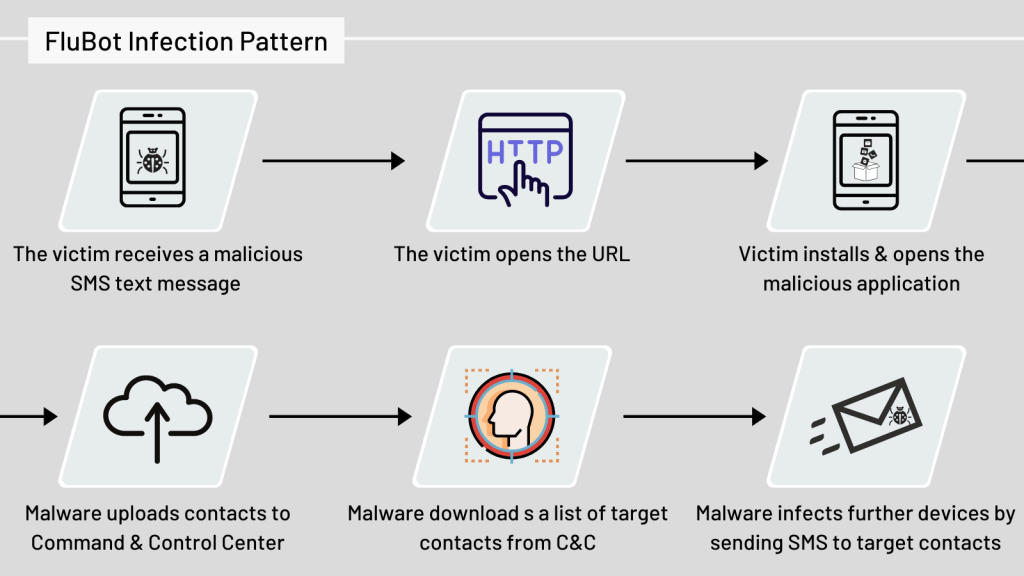
\includegraphics[scale=0.41]{command_control_server.png}\footnote{threatmark.com}
\end{frame}

\begin{frame}{Phishing Methoden}
\begin{itemize}
 \item Anfangs wird eine vermeintliche Voicemail als Köder verwendet
 \item Seit Frühjahr 2021 vermehrt Packerlieferdienste
 \item Ab mitte 2021 'Fake security patches' gegen Flubot selbst
 \item Anfang 2022 nun Adobe Apps
 \item Flubot variert und wechselt häufig Phishing Köder! 
\end{itemize}


\end{frame}
\begin{frame}
\begin{center}
 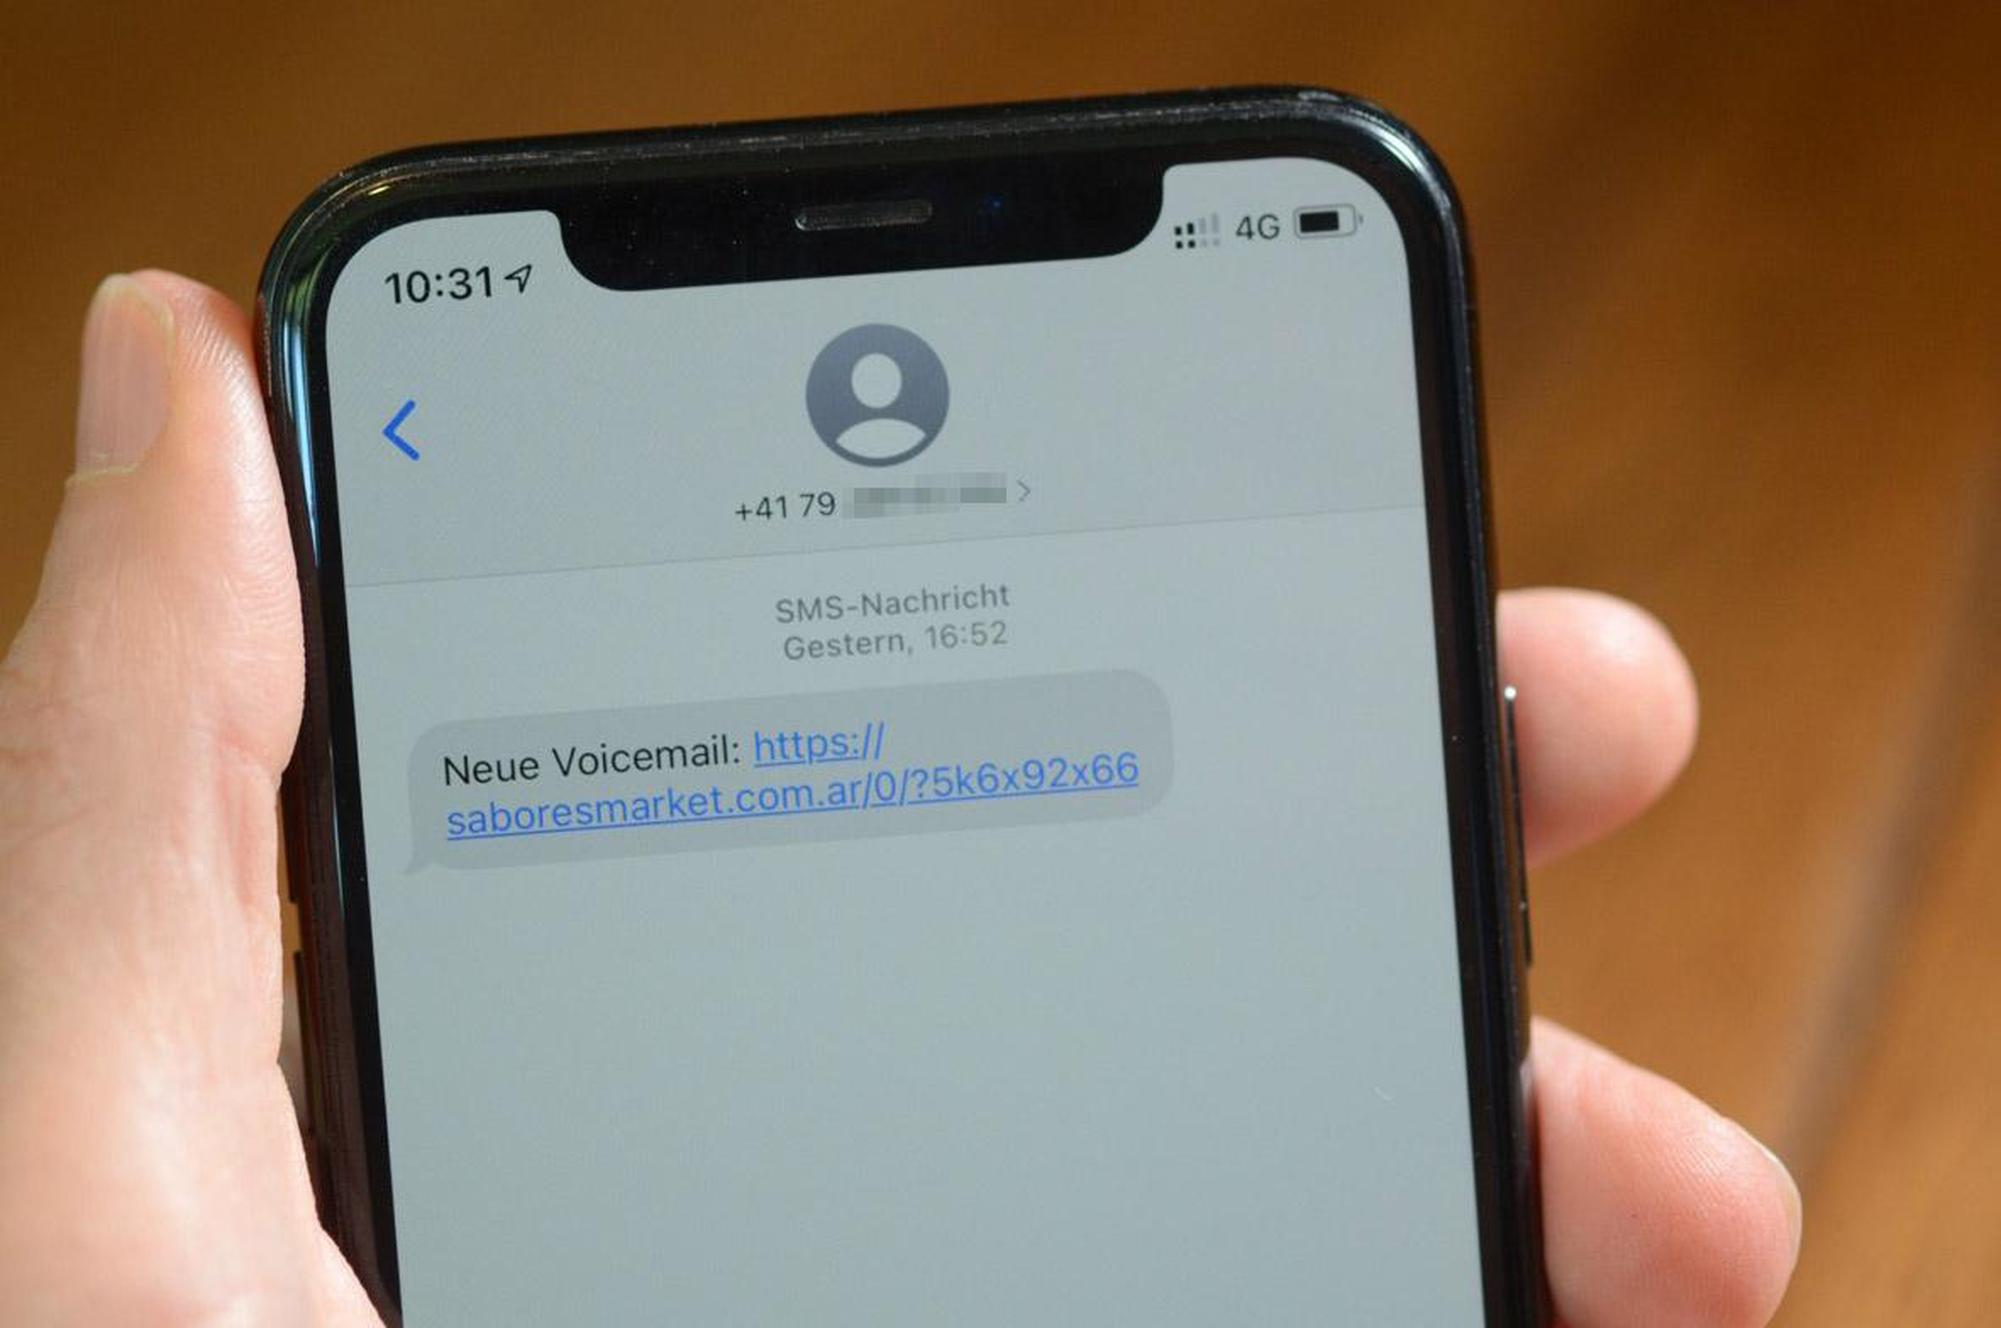
\includegraphics[scale=0.15]{firstvoice.jpg}\footnote{threatmark.io}

\end{center}


\end{frame}


\begin{frame}
\begin{center}
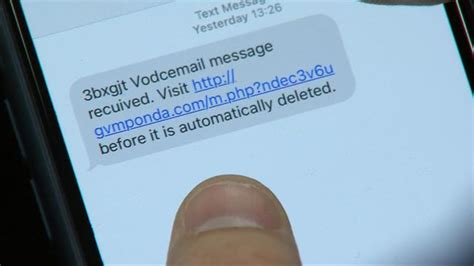
\includegraphics[scale=0.51]{voice.jpeg}\footnote{bsi.de}

\end{center}
\end{frame}
\begin{frame}
\begin{center}
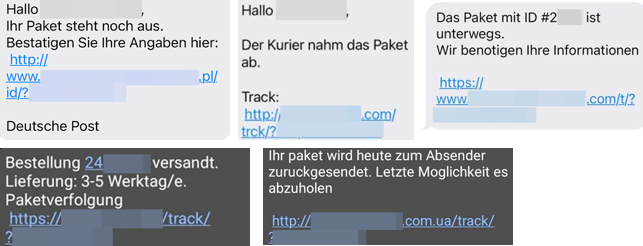
\includegraphics[scale=0.51]{external-content.duckduckgo.com.png}\footnote{computerbild.de}

\end{center}


\end{frame}
\begin{frame}
\begin{center}
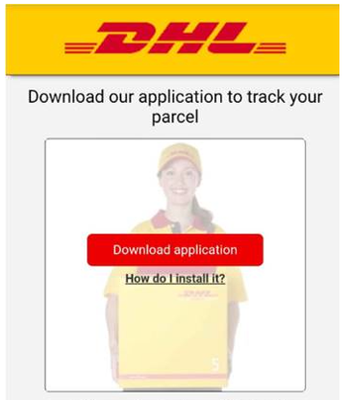
\includegraphics[scale=0.51]{dhl.png}\footnote{threatmonit.io}

\end{center}


\end{frame}
\subsection{Post-Infection}
\begin{frame}{Post-Infection}
 \begin{itemize}
  \item Verbindungsaufbau zum Command and Control Server
 \end{itemize}

\begin{block}{Command and Control Server}
Hauptzentrale des Botnetzes! Hier wird die Malware gesteuert!
\end{block}
\begin{itemize}
 \item Gerät schickt alle Kontakte und installierten Apps an den C\&C Server!
\item Dieser antwortet mit einer neuen Liste neuer Kontakte\\
$\Rightarrow$ Über diese werden weitere Phishing SMS versendet!
\item Zudem wird eine Liste der geziehlten Anwendungen geschickt
\item Über diese Anwendungen wird nun das eigentliche Phishing Overlay gelegt!
 \end{itemize}

\end{frame}
\begin{frame}
\begin{center}
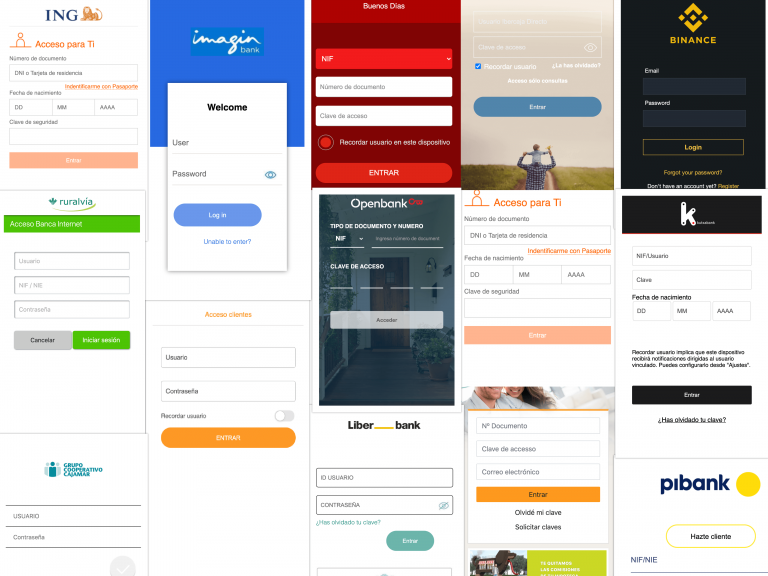
\includegraphics[scale=0.51]{infected.png}\footnote{threatmark.io}

\end{center}


\end{frame}
\section{Technische Analyse}
\begin{frame}{Technische Analyse}
\begin{itemize}
 \item Die Malware APK ist komplett in Java geschrieben
 \item Läuft ab Android Version 4.1.2
 \item Wird stetig weiterentwickelt
 \item Verwendung von String Obfuscation um Reverse Engineering zu erschweren!
 \item Über 30 Kommandos für Kommunikation zwischen Gerät und C\&C möglich!
\end{itemize}
\end{frame}
\begin{frame}{Command and control Server}
 \begin{itemize}
  \item Hauptzentrale der Malware Infrastruktur
  \item Bietet Angreifern Administration
  \item Server - Client model
  \item Über 20 Kommandos zwischen Gerät und C\&C möglich
  \item Zugreifbar über Weboberfläche
  \item Liegt in einem verteilten System
 \end{itemize}

\end{frame}
\begin{frame}
\begin{center}
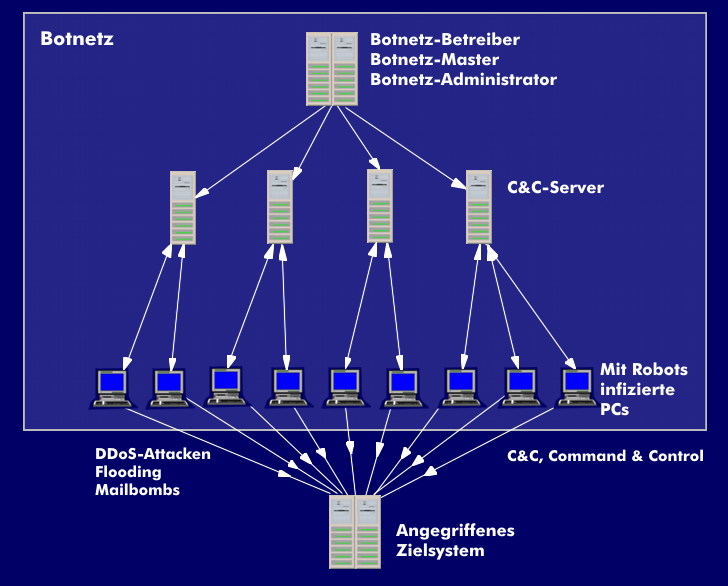
\includegraphics[scale=0.51]{comand.png}\footnote{heise.de}

\end{center}


\end{frame}


\begin{frame}
\begin{shaded}
\#Kommandos von dem C\&C Server an das Gerät

GET\_CONTACTS - Schicke Kontakte an den Server.\\
RETRY\_INJECT - Versuche erneut die Anwendung zu infizieren\\
BLOCK - Jegliche Kommunikation blocken\\
UNINSTALL\_APP - Deinstalltion der Malware\\
SEND\_SMS - Versenden von SMS\\
DISABLE\_PLAY\_PROTECT - Den Virenschutz des Google Play stores deaktivieren\footnote{https://raw.githubusercontent.com/prodaft/malware-ioc/master/FluBot/FluBot.pdf}
\end{shaded}
\end{frame}

\begin{frame}{Netzwerkstrukur}
\begin{itemize}
 \item Flubot verwendet gekapperte Webeiten als Hosts für C\&C
 \item Mehrere hundert betroffene Instanzen\\
 - meist Wordpress Blogs\\
 - stetig wachsend
 \item Keine feste Domain oder IP
 \item Stattdessen Domaingenerierung anhand des Domain-Generation-Algorithmus
 \end{itemize}



- Auflösung über DNS über HTTPS\\
- Nutzt Services wie dns.google
\end{frame}
\begin{frame}{Domain Generation Algorithmus}
 Algorithmus zu Domain Generierung
 \begin{itemize}
 \item Kombiniert randomisiert Top-Level-Domain mit Second-Level-Domain
 \item Liste 1 enthält Top-Level-Domains\\
 \[.de, .com, .net, .org, .io\]
 \item Liste 2 enthält Second-Level-Domains\\
 \[test, hallowelt, Albstat, Lirum, Ipsum\]
 \item Aus diesen Listen werden nun versucht vollständige Domains aufzulösen
 \end{itemize}

\end{frame}
\begin{frame}
 \begin{itemize}
  \item Für die Domainauflösung werden Dienste von google oder cloudflare genutzt\\
  $\Rightarrow$ dns.google, cloudflare.dns
  \item Teilweise werden bis zu 10 DNS Requests benötigt 
 \end{itemize}

\end{frame}

\begin{frame}
\begin{center}
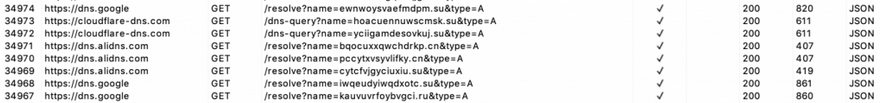
\includegraphics[scale=0.51]{dns.png}\footnote{threatmark.io}

\end{center}
\end{frame}
\section{Lösungen}
\begin{frame}{Lösungsansätze}
 \begin{itemize}
  \item Enfernung der Malware durch Rücksetzung zum Werkszustand möglich
  \item Verlust der Persönlichen Daten zur Folge
  \item Open-Source tools wie paranoid bieten ALternative
  \item Gegen Phishing Angriffe kaum technische Lösungen vorhanden
  \item Zwei-Faktor-Authentifizierung bietet gewissen Schutz
  \item Bildung bietet größte Chance\\
  $\Rightarrow$ Informatik in Schulen kaum Schwerpunkt
  \item Umgang mit digitalen Medien sollte Flächendeckend gelehrt werden
 \end{itemize}

\end{frame}

\section{Conclusion und Ausblick}
\begin{frame}{Conclusion und Ausblick}
\begin{itemize}
 \item Phishing nach wie vor eine der größten Bedrohungslagen
 \item Meist in Verbindung mit weiterer Malware eingesetzt
 \item Android häufigstes Zielsystem
 \item 'Internet of things' vergrößert Angriffsziele
 \item Technologien wie nfts, smartcontracts könnten abhilfe schaffen
 \item Nachhaltiger Schutz bzw. Bekämpfung nur durch bessere Aufklärung und Bildung möglich
\end{itemize}
\end{frame}
\section{Quellen}
\begin{frame}{Quellen}
computerbild | 07.11.2021, https://www.computerbild.de/artikel/cb-News-Sicherheit-Flubot-Gefaehrliche-Android-Malware-verbreitet-sich-ueber-Fake-Patches-30863335.html\\

threatmark | 07.01.2022, https://www.threatmark.com/flubot-banking-malware\\

threadmonit | 06.01.2022, https://www.threatmonit.io/flubot-android-malware-technical-analysis\\

heise | 02.01.2022, https://www.heise.de/news/Smishing-BSI-warnt-vor-neuen-Betrugsmaschen-bei-SMS-Phishing-6220072.html\\

bsi | 03.01.2022, https://www.bsi.bund.de/DE/Themen/Verbraucherinnen-und-Verbraucher/Cyber-Sicherheitslage/Methoden-der-Cyber-Kriminalitaet/Botnetze/Steckbriefe-aktueller-Botnetze/Steckbriefe/Flubot.html\\ 

\end{frame}
\begin{frame}
 https://de.statista.com/statistik/daten/studie/1235321\\
https://de.statista.com/themen/1355/android/\\
https://www.telekom.com/en/blog/group/article/flubot-under-the-microscope-636368\\
https://www.telekom.com/en/blog/group/article/flubot-under-the-microscope-636368\\
https://www.computerbild.de/artikel/cb-News-Sicherheit-Flubot-Gefaehrliche-Android-Malware-verbreitet-sich-ueber-Fake-Patches-30863335.html\\
https://computerwelt.at/news/android-malware-flubot-stuermt-top-ten\\
https://www.telekom.com/en/blog/group/article/flubot-under-the-microscope-636368\\
\end{frame}




\end{document}
